\documentclass{article}
\usepackage{graphicx}
\usepackage[margin=1.5cm]{geometry}
\usepackage{amsmath}

\begin{document}
\twocolumn

\title{Wednesday Warm Up: Unit 6: Fixed axis rotation}
\author{Prof. Jordan C. Hanson}

\maketitle

\section{Memory Bank}

\begin{itemize}
\item $\vec{s} = \vec{\theta} \times \vec{r}$ ... Geometric relationship.
\item $\vec{v} = \vec{\omega} \times \vec{r}$ ... Geometric relationship.
\item $\vec{\tau} = \vec{r} \times \vec{F}$ ... The relationship between \textit{torque}, $\vec{\tau}$, the \textit{moment arm}, $\vec{r}$, and the \textit{force}, $\vec{F}$.
\item $\vec{\tau} = I \vec{\alpha}$ ... Newton's 2nd law, in angular form.
\item $W = \vec{\tau} \cdot \vec{\theta}$ ... Definition of work, angular form.
\item $d\vec{L}/dt = \vec{\tau}$ ... Newton's 2nd law in angular form, with angular momentum.
\end{itemize}

\section{Fixed Axis Rotation, Torque, and Kinetic Energy}

\begin{enumerate}
\item An aircraft is coming in for a landing at 300 meters height when the propeller falls off. When it comes off, the propeller has a rotation rate of 20 rev/s, a moment of inertia of 70.0 kg m$^2$, and a mass of 200 kg. If air resistance is present and reduces the propeller’s rotational kinetic energy at impact by 30\%, what is the propeller’s rotation rate at impact? \\ \vspace{3cm}
\item A neutron star of mass $2\times 10^{30}$ kg and radius 10 km rotates with a period of 0.02 seconds. (a) What is its rotational kinetic energy? (b) If, 10 years later, a period of 0.04 seconds is observed, what energy was lost? (c) What is loss rate (power) that caused the slowdown? \\ \vspace{3cm}
\item Using $d\vec{L}/dt = \vec{\tau}$, show qualitatively that when a bicyclist leans left, he turns left. \\ \vspace{6cm}
\item If $\vec{\tau} = 0$, explain why angular momentum is conserved.
\end{enumerate}

\begin{figure}
\centering
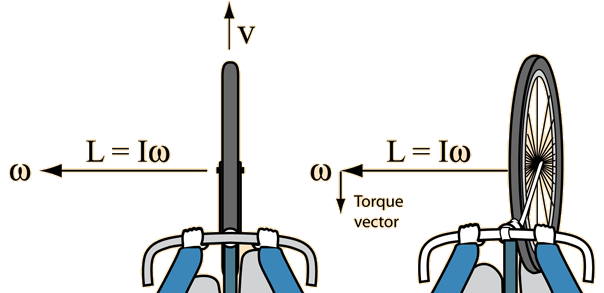
\includegraphics[width=0.4\textwidth]{figures/bike2.png}
\caption{\label{fig:1} A bicycle turns left if you lean left.}
\end{figure}

\end{document}
